\documentclass[11pt,letterpaper]{article}

% ── Packages ────────────────────────────────────────────────────────────────
\usepackage[margin=1in]{geometry}
\setlength{\headheight}{22pt}
\addtolength{\topmargin}{-10pt}
\usepackage{mathptmx}
\usepackage{amsmath,amssymb,amsthm}
\usepackage{booktabs}
\usepackage{graphicx}
\usepackage{tikz}
\usetikzlibrary{arrows.meta,positioning,shapes.geometric,fit,calc,backgrounds}
\usepackage{xcolor}
\usepackage{hyperref}
\usepackage{enumitem}
\usepackage{titlesec}
\usepackage{caption}
\usepackage{array}
\usepackage{microtype}
\usepackage{fancyhdr}

% ── Colors ──────────────────────────────────────────────────────────────────
\definecolor{econblue}{RGB}{20,55,95}
\definecolor{softgray}{RGB}{95,95,95}
\definecolor{boxfill}{RGB}{245,247,250}
\definecolor{boxedge}{RGB}{40,70,110}
\definecolor{arrowcol}{RGB}{50,70,100}
\definecolor{lightline}{RGB}{200,205,215}

\hypersetup{
  colorlinks=true,
  linkcolor=econblue,
  citecolor=econblue,
  urlcolor=econblue,
  pdftitle={Synthetic Cultural Agents 2.0: Beyond Persona-Prompting},
  pdfauthor={Augusto Gonzalez-Bonorino and Kseniia Biriukova}
}

% ── Typography ──────────────────────────────────────────────────────────────
\titlespacing*{\section}{0pt}{0.9em}{0.35em}
\titlespacing*{\subsection}{0pt}{0.7em}{0.25em}
\titleformat{\section}{\large\bfseries\color{econblue}}{\thesection.}{0.6em}{}
\titleformat{\subsection}{\normalsize\bfseries\color{econblue}}{\thesubsection}{0.5em}{}
\setlist[itemize]{leftmargin=1.4em,itemsep=0.15em,topsep=0.2em}
\setlist[enumerate]{leftmargin=1.5em,itemsep=0.15em,topsep=0.2em}
\captionsetup{font=small,labelfont={bf,color=econblue},skip=3pt}
\setlength{\parskip}{0.28em}
\setlength{\parindent}{1.1em}

% ── Header / footer ─────────────────────────────────────────────────────────
\pagestyle{fancy}
\fancyhf{}
\fancyhead[L]{\small\color{softgray} EconLLM Lab · SCA 2.0 Position Paper}
\fancyhead[R]{\small\color{softgray}\thepage}
\renewcommand{\headrulewidth}{0.3pt}
\renewcommand{\headrule}{\hbox to\headwidth{\color{lightline}\leaders\hrule height \headrulewidth\hfill}}
\fancypagestyle{plain}{%
  \fancyhf{}%
  \fancyfoot[C]{\small\color{softgray}\thepage}%
  \renewcommand{\headrulewidth}{0pt}%
}

% ── Helpers ─────────────────────────────────────────────────────────────────
\newcommand{\GPS}{\textsc{gps}}
\newcommand{\WVS}{\textsc{wvs}}
\newcommand{\DPO}{\textsc{dpo}}
\newcommand{\SCA}{\textsc{sca}}
\newcommand{\LLM}{\textsc{llm}}
\newcommand{\WEIRD}{\textsc{weird}}
\newcommand{\LoRA}{\textsc{lora}}

\begin{document}

% ════════════════════════════════════════════════════════════════════════════
% COVER
% ════════════════════════════════════════════════════════════════════════════
\thispagestyle{empty}
\begin{center}
{\color{econblue}\rule{\textwidth}{1.1pt}}\\[0.3em]
{\LARGE\bfseries\color{econblue} Synthetic Cultural Agents 2.0:}\\[0.15em]
{\LARGE\bfseries\color{econblue} Beyond Persona-Prompting}\\[0.3em]
{\color{econblue}\rule{\textwidth}{0.55pt}}\\[0.55em]

{\normalsize A Position Paper on Structural Preference Estimation
for Culturally Aligned Language Models}\\[0.7em]

{\large\textbf{Augusto Gonzalez-Bonorino}\textsuperscript{1}
\quad and\quad
\textbf{Kseniia Biriukova}\textsuperscript{2}}\\[0.35em]

{\small\textsuperscript{1}Department of Economics, Arizona State University; EconLLM Lab.
Correspondence: \texttt{agonz439@asu.edu}.}\\[0.1em]
{\small\textsuperscript{2}EconLLM Lab; preference fine-tuning and evaluation pipeline.}\\[0.35em]

{\normalsize August 2026 \quad·\quad
\textit{Working document --- position paper \& empirical results}}\\[0.35em]
{\color{econblue}\rule{0.3\textwidth}{0.35pt}}
\end{center}

\vspace{0.25em}
\noindent
{\footnotesize\color{softgray}
\textbf{Status.} Intermediate summary of SCA~2.0: structural conjecture, implemented DPO pipeline, Tier-1 synthetic pair recovery, and Tier-2 out-of-sample empirical evaluation on World Values Survey Wave~7 items ($N=35$). Code \& data: \href{https://github.com/EconLLM-Lab/SCA2_PofW}{\texttt{github.com/EconLLM-Lab/SCA2\_PofW}}.\par
}

\vspace{0.4em}

% ════════════════════════════════════════════════════════════════════════════
\section*{Abstract}

Large language models are increasingly used as simulators of human judgment in economics and adjacent social sciences, yet their default alignment reflects predominantly Western, Educated, Industrialized, Rich, and Democratic (\WEIRD{}) preference data. Earlier Synthetic Cultural Agents (\SCA{}~1.0) addressed this gap by conditioning frontier models on ethnographic profiles at inference time. That approach is useful for piloting but is reduced-form: cultural signal lives only in the prompt, is fragile to model updates, and does not support formal identification or counterfactual analysis.

This position paper outlines \SCA{}~2.0, a structural alternative. We treat Direct Preference Optimization (\DPO{}) as maximum-likelihood estimation in a Bradley--Terry random-utility model, using the Global Preferences Survey (\GPS{}) six-dimensional cultural state vector to generate culture-conditioned synthetic preference data. A student model (\texttt{Llama-3.1-8B-Instruct}) is fine-tuned via QLoRA with unconditioned prompts (\texttt{PROMPT\_COUNTRY\_CONDITIONING = False}) so that cultural dispositions are encoded into parameters rather than transient context. 

We evaluate the framework across two tiers: (i)~Tier-1 synthetic pair recovery ($n=200$), where own-country adapters achieve $70.0$--$78.5\%$ accuracy; and (ii)~Tier-2 empirical out-of-sample evaluation on $N=35$ unseen World Values Survey (WVS) Wave~7 items mapped to GPS dimensions. On non-\WEIRD{} targets (Mexico), the matched MEX adapter demonstrates strong cultural specificity, outperforming the cross USA adapter on $97.1\%$ of questions ($\Delta\text{TVD} = 0.1495$, $95\%$ CI: $[0.0964, 0.2152]$). Conversely, on US targets, the USA adapter suffers from collision with the base model's strong American pretraining prior. Option log-likelihood scoring exhibits systematic under-dispersion relative to human populations. We formalize the measurement argument through a Cronbach--Meehl nomological network linking the \GPS{} source instrument, the DPO training domain, and the WVS criterion domain, and we delineate reliable applications (relative comparative statics, pre-field instrument stress-testing) from unreliable ones (absolute headcount polling, fine-tuning over already-dominant priors).

\vspace{0.4em}
\noindent\textit{Keywords:} cultural preferences; Direct Preference Optimization; Bradley--Terry; Global Preferences Survey; structural estimation; construct validity; World Values Survey

% ════════════════════════════════════════════════════════════════════════════
\section{Introduction}

Social scientists increasingly use large language models (\LLM{}s) as low-cost simulators of survey responses, experimental subjects, and policy interlocutors. The practical appeal is clear: a model can generate thousands of responses in minutes, enabling exploratory design work before expensive fieldwork. The scientific risk is equally clear. Preference fine-tuning and human feedback data for frontier models are concentrated in \WEIRD{} populations \cite{henrich2010,falk2018}. When a model is asked to ``answer as someone in Lagos, Buenos Aires, or Mexico City,'' its behavior still largely reflects that default alignment---unless culture is introduced in a disciplined way.

The first generation of Synthetic Cultural Agents \cite{capra2025} showed that persona prompting---conditioning a frontier model on demographic and ethnographic profiles---can reproduce non-\WEIRD{} patterns in economic experiments to a surprising degree. For piloting and hypothesis generation, that result is valuable. Methodologically, however, persona prompting is a reduced-form intervention. Cultural information lives in the context window; it vanishes when the session ends; and it provides no structural object (preferences, technology, information) that can be identified, tested, or counterfactually varied.

\SCA{}~2.0 reframes the problem as structural preference estimation. The core conjecture is:

\begin{quote}
\textit{Cultural preferences measured by the Global Preferences Survey can be encoded into language-model policies via preference fine-tuning, so that implied utilities recover the direction of culture-conditioned choices and support formal evaluation against independent survey moments.}
\end{quote}

Three features distinguish the program from prompt engineering. First, culture is parameterized by an externally measured vector---the six \GPS{} dimensions of Falk et al.\ \cite{falk2018}---rather than by free-form narrative alone. Second, training uses Direct Preference Optimization \cite{rafailov2023}, which is mathematically a reparameterization of Bradley--Terry maximum likelihood \cite{bradley1952,mcfadden1974}; this licenses econometric language (utility, identification, overidentification) with minimal translation cost. Third, validation is hierarchical: \GPS{}-targeted synthetic pairs identify the cultural state; World Values Survey (\WVS{}) items are reserved for out-of-sample evaluation; held-out behavioral tasks assess generalization.

This document serves as both a position paper and a report on completed out-of-sample empirical evaluations on WVS Wave~7 data. Its goals are to (i)~state the conjecture and design cleanly, (ii)~present an honest reading of Tier-1 and Tier-2 empirical evaluations, (iii)~frame construct validity for latent cultural variables in LLMs, and (iv)~demarcate reliable applications from invalid downstream uses.

% ════════════════════════════════════════════════════════════════════════════
\section{Related Work}

Three short literatures motivate the design.

The \GPS{} \cite{falk2018} supplies incentivized measures of patience, risk taking, positive and negative reciprocity, altruism, and trust across 76 countries---a low-dimensional, cross-culturally comparable parameter vector. Country means are not individuals (within-country variance is often large), but they are a defensible starting point for population-level simulation. A growing experimental literature uses \LLM{}s as simulated respondents \cite{horton2023,achar2023}; much of it is reduced-form role prompting, the family to which \SCA{}~1.0 belongs. Complementary work documents cultural gaps in model outputs \cite{cao2023,durmus2024} but typically stops at evaluation rather than estimation. \DPO{} \cite{rafailov2023} optimizes a policy so preferred responses receive higher probability than dispreferred ones relative to a reference model; under standard assumptions this coincides with Bradley--Terry likelihood for a scaled log-probability score---the bridge to structural econometrics.

What is missing---and what \SCA{}~2.0 targets---is a pipeline that grounds preference data in an external cultural instrument, fine-tunes open-weight models rather than relying on prompts alone, and subjects the resulting agents to rigorous out-of-sample evaluation.

% ════════════════════════════════════════════════════════════════════════════
\section{Methodology}

\subsection{Primitives}

Let $x$ denote a decision scenario (prompt) and $y$ a free-text response. A cultural state is a vector
\begin{equation}
  z = \bigl(\delta,\ \gamma,\ \xi^{+},\ \xi^{-},\ \alpha,\ \tau\bigr)^{\!\top}
  \in \mathbb{R}^{6},
\end{equation}
corresponding to time preference (patience), risk taking, positive reciprocity, negative reciprocity, altruism, and trust from the \GPS{}. An \SCA{} is a policy $\pi(\cdot\mid x; z)$ whose behavior is governed by a separable reward
\begin{equation}
  R(x,y;z) \;=\; r_{\mathrm{task}}(x,y) \;+\; \phi(z)^{\!\top} m(x,y),
  \label{eq:reward}
\end{equation}
where $r_{\mathrm{task}}$ captures generic competence (coherence, relevance), $m(x,y)\in\mathbb{R}^{6}$ is a vector of measurable behavioral features of the response, and $\phi:\mathbb{R}^{6}\to\mathbb{R}^{6}$ maps \GPS{} scores into reward weights.

\paragraph{The structural assumption.}
Equation~\eqref{eq:reward} is a \emph{structural} (not descriptive) assumption: it claims that the country-specific component of an agent's behavior is a linear function of six externally measured preference traits, mediated by observable features of the response. Two testable implications follow. First, \emph{separability}: the task term $r_{\mathrm{task}}$ is country-invariant, so any cross-country behavioral difference must load on $\phi(z)^{\!\top} m(x,y)$. Second, \emph{dimensional structure}: only six dimensions of cultural variation are permitted to matter. Both implications are falsifiable---the first by the matched-versus-cross specificity design (Section~4), the second by out-of-sample items that ``should not'' be explained by any dimension and by items whose loading is measured rather than imposed.

\subsection{Choice model}

We treat the agent's response as a discrete choice over a finite option set $\mathcal{Y} = \{y_1,\dots,y_K\}$ (the response codes of a survey item or the two completions of a preference pair). A Luce--Bradley--Terry--McFadden random-utility model sets
\begin{equation}
  \Pr(y_k \mid x; z) \;=\;
  \frac{\exp\bigl(R(x,y_k;z)\bigr)}{\sum_{j=1}^{K}\exp\bigl(R(x,y_j;z)\bigr)},
  \label{eq:choice}
\end{equation}
which is the softmax over option rewards. For a pair $\{y^{w}, y^{\ell}\}$, equation~\eqref{eq:choice} collapses to the familiar logistic paired-comparison probability
\begin{equation}
  \Pr(y^{w}\succ y^{\ell}\mid x) \;=\;
  \sigma\bigl(R(x,y^{w};z)-R(x,y^{\ell};z)\bigr),
  \label{eq:bt}
\end{equation}
with $\sigma(u) = (1+e^{-u})^{-1}$.

Equation~\eqref{eq:choice} is the exact object the evaluation pipeline estimates: the option-likelihood protocol (Section~4) computes $\hat{p}_k \propto \exp(\text{logprob}(y_k\mid x))$ over all valid response codes and compares the resulting distribution to the empirical population distribution. The LLM is therefore used as a \emph{choice-probability simulator}, not a text generator---a deliberate design choice that makes the model's output directly comparable to the random-utility object in equation~\eqref{eq:choice}.

\subsection{DPO as structural estimation}

Given preference data $\{(x_i,y_i^{w},y_i^{\ell})\}_{i=1}^{n}$ in which $y^{w}$ is preferred to $y^{\ell}$ under cultural state $z$, the Bradley--Terry likelihood is
\begin{equation}
  \mathcal{L}(R) \;=\;
  \prod_{i=1}^{n} \sigma\bigl(R(x_i,y_i^{w};z)-R(x_i,y_i^{\ell};z)\bigr).
  \label{eq:likelihood}
\end{equation}
Direct Preference Optimization \cite{rafailov2023} maximizes this likelihood while reparameterizing the reward difference through the log-ratio of the trained policy to a frozen reference policy:
\begin{equation}
  R(x,y_1;z)-R(x,y_2;z)
  \;=\;
  \beta\left[
    \log\frac{\pi_{\theta}(y_1\mid x)}{\pi_{\mathrm{ref}}(y_1\mid x)}
    -
    \log\frac{\pi_{\theta}(y_2\mid x)}{\pi_{\mathrm{ref}}(y_2\mid x)}
  \right],
  \label{eq:logratio}
\end{equation}
where $\pi_{\mathrm{ref}}$ is a frozen reference model and $\beta>0$ is a scale temperature. Equation~\eqref{eq:logratio} is the empirical analogue of the structural reward in equation~\eqref{eq:reward}: after training, the analyst can compute, for any held-out pair, the \emph{implied reward margin} $\widehat{\Delta r} = \beta\,[\text{log-ratio of chosen} - \text{log-ratio of rejected}]$, which is the estimated utility difference under the country-specific $z$.

\paragraph{Identification and its limits.}
Equation~\eqref{eq:logratio} identifies reward \emph{differences} up to scale ($\beta$) and location (any additive constant cancels in paired comparisons). The two structural features we \emph{can} recover are (i)~the sign of $\Delta r$---which option a country's policy ranks higher---and (ii)~the own-versus-other contrast, i.e., whether an adapter trained on country $c$'s labels assigns systematically larger margins to $c$'s chosen options than an adapter trained on country $c'$. We cannot recover the absolute level of $R$ nor, in general, the individual coordinates of $\phi(z)$ without additional moment conditions---a limitation we make explicit rather than obscure.

\subsection{Pipeline Architecture}

Figure~\ref{fig:pipeline} summarizes the pipeline architecture across data generation, fine-tuning, and out-of-sample validation.

\begin{figure}[t]
\centering
\begin{tikzpicture}[
  font=\scriptsize,
  node distance=0.42cm and 0.28cm,
  box/.style={
    draw=boxedge, fill=boxfill, rounded corners=2pt,
    align=center, inner sep=4pt, text width=2.15cm, minimum height=1.05cm,
    line width=0.6pt
  },
  smallbox/.style={
    draw=boxedge, fill=white, rounded corners=2pt,
    align=center, inner sep=3pt, text width=1.85cm, minimum height=0.72cm,
    line width=0.5pt
  },
  arr/.style={-{Stealth[length=2.2mm]}, color=arrowcol, line width=0.7pt},
  lab/.style={font=\tiny\color{softgray}, align=center}
]

\node[box] (A) {\textbf{A. Cultural state}\\$z_c$ from \GPS{}\\+ ethnographic profile};
\node[box, right=of A] (B) {\textbf{B. Scenarios}\\5 facets $\times$ dim\\country-neutral prompts};
\node[box, right=of B] (C) {\textbf{C. Preference pairs}\\fixed high/low options\\country selects chosen};
\node[box, right=of C] (D) {\textbf{D. Quality control}\\6-dim scoring\\mono / distance / contamination};
\node[box, right=of D] (E) {\textbf{E. Student \DPO{}}\\open-weight +\LoRA{}\\implied reward recovery};

\draw[arr] (A) -- (B);
\draw[arr] (B) -- (C);
\draw[arr] (C) -- (D);
\draw[arr] (D) -- (E);

\node[lab, below=0.12cm of A] {identification\\input};
\node[lab, below=0.12cm of B] {shared design};
\node[lab, below=0.12cm of C] {labels from $z_c$};
\node[lab, below=0.12cm of D] {retain + label};
\node[lab, below=0.12cm of E] {structural\\estimation};

% validation branch
\node[smallbox, below=1.15cm of C] (V1) {Tier 1: Implied $\Delta r$\\on held-out synthetic\\pairs (executed)};
\node[smallbox, right=0.55cm of V1] (V2) {Tier 2: \WVS{} Wave 7\\OOS option likelihood\\(executed)};
\node[smallbox, left=0.55cm of V1] (V3) {Tier 3: Task\\generalization\\(planned)};

\draw[arr] (E.south) -- ++(0,-0.35) -| (V1.north);
\draw[arr] (V1) -- (V2);
\draw[arr, dashed] (V1) -- (V3);

\node[lab, below=0.08cm of V2] {empirical OOS};
\node[lab, below=0.08cm of V3] {generalization};

\end{tikzpicture}
\caption{SCA~2.0 pipeline architecture. Solid lines mark executed pipeline stages. Culture enters as an external \GPS{} vector $z_c$; synthetic pairs are generated, quality-controlled, and fine-tuned via \DPO{}; model validation proceeds through Tier-1 synthetic pair recovery and Tier-2 empirical WVS Wave~7 option-likelihood evaluation.}
\label{fig:pipeline}
\end{figure}

\subsection{Construct validity and the nomological network}

Because $z$ is a \emph{latent} construct---nobody observes ``patience in Mexico'' directly---the scientific status of the pipeline hinges on construct validity. We adopt the classical formulation of Cronbach and Meehl \cite{cronbach1955}: a construct is validated by embedding it in a \emph{nomological network}, a set of theoretical relations linking the construct to (a)~other constructs and (b)~observable measures. Validation is then a matter of testing whether the observed correlations behave as the network predicts.

\paragraph{The network.}
For the latent construct ``country-level economic preference disposition,'' the network has three nodes---three families of observables that the construct must systematically relate to:

\begin{enumerate}[leftmargin=1.5em]
  \item \textbf{Source domain (identification):} the \GPS{} instrument $z_c$ (Falk et al., 2018), an incentivized, cross-nationally comparable measure of the six preference dimensions. This is the \emph{defining} measure of the construct: $z_c$ is what we mean by ``Mexico's preference profile'' in this paper.
  \item \textbf{Training domain (internal manifestation):} the synthetic preference pairs $\{(x_i, y_i^w, y_i^\ell)\}$ whose labels are generated by $z_c$, and the implied reward margins $\widehat{\Delta r}$ recovered from the trained policy.
  \item \textbf{Criterion domain (external manifestation):} the World Values Survey (WVS) item-response distributions $P_{\mathrm{WVS}}$, an independent, human-administered survey that was \emph{not} used in training and whose items are mapped to the six dimensions via a curated schema (\texttt{question\_map\_wvs\_edited.csv}).
\end{enumerate}

The network postulates three links, each with a distinct falsifiable prediction:

\begin{enumerate}[leftmargin=1.5em]
  \item \textbf{Link 1 (source $\rightarrow$ training):} preferences implied by $z_c$ must rank $y^w$ above $y^\ell$ on held-out pairs. Falsified if the trained policy fails to recover its own labels (Tier-1 preference accuracy $\leq 0.5$).
  \item \textbf{Link 2 (training $\rightarrow$ criterion, convergent validity):} an adapter trained on $z_c$ must reduce distributional error against $P_{\mathrm{WVS}}$ for country $c$ on unseen items, relative to the base model---because both the synthetic labels and the WVS responses are driven by the same underlying $z_c$. Falsified if fine-tuning does not improve (or degrades) empirical fit.
  \item \textbf{Link 3 (criterion-domain discrimination, discriminant validity):} an adapter trained on $z_{c}$ must fit $c$'s WVS distributions better than an adapter trained on $z_{c'}$, on the \emph{same} items, with country names withheld from the prompt. Falsified if the matched adapter does not dominate the cross adapter (matched-vs-cross specificity $\leq 0.5$).
\end{enumerate}

\paragraph{How the network handles negative evidence.}
The network is a \emph{joint} claim, and its links can fail independently---which is precisely what the data show. The USA adapter \emph{passes} Link~1 (Tier-1 accuracy $0.70$) but \emph{fails} Links~2--3 on US WVS items: the base model already encodes a strong US pretraining prior, so the adapter's additional synthetic signal over-corrects rather than refines. This is not evidence against the construct; it is evidence that the \emph{source domain} is redundant with the model's pretraining for WEIRD populations. The same network then correctly predicts that the MEX adapter---trained on a population outside the pretraining prior---should pass all three links, which it does (Tier-1 accuracy $0.785$; matched-vs-cross specificity $97.1\%$ on MEX items; dimension-level convergence such as Altruism TVD falling from $0.450$ to $0.152$).

\paragraph{Reliability.}
Reliability---consistency of measurement---is assessed within the same framework: bootstrap confidence intervals over questions (2,000 replications) for every reported metric; calibration tables (predicted versus empirical option frequencies, ECE); and signed moment diagnostics (mean and dispersion bias) that reveal the structural under-dispersion of softmax option scoring. These diagnostics do not merely qualify the results; they are part of the nomological network, because they bound how much of the observed fit is construct signal versus scoring artifact.

% ════════════════════════════════════════════════════════════════════════════
\section{Empirical Results}

\subsection{Tier-1: Synthetic Preference Recovery}

Table~\ref{tab:main} reports Tier-1 results on held-out synthetic preference pairs ($n=200$ per adapter--country cell). Both the Mexico and US adapters recover their own culture-conditioned synthetic labels well above chance ($78.5\%$ and $70.0\%$ preference accuracy, respectively), while cross-country accuracy remains near chance ($52.0\%$ and $45.5\%$).

\begin{table}[h!]
\centering
\caption{Tier-1 Cross-evaluation of country adapters on held-out synthetic preference pairs ($n=200$ per cell). Preference accuracy is the share of pairs with positive implied reward margin ($\Delta r > 0$).}
\label{tab:main}
\scriptsize
\begin{tabular}{@{}ll rrrr@{}}
\toprule
\textbf{Adapter} & \textbf{Eval Data} & \textbf{$n$} & \textbf{Mean $\Delta r$} & \textbf{Pref.\ Accuracy} & \textbf{Mean $P(\mathrm{chosen})$} \\
\midrule
Mexico Adapter & Mexico & 200 & $+1.70$ & $0.785$ & $0.714$ \\
Mexico Adapter & United States & 200 & $-0.22$ & $0.520$ & $0.501$ \\
USA Adapter & Mexico & 200 & $-0.20$ & $0.455$ & $0.464$ \\
USA Adapter & United States & 200 & $+0.78$ & $0.700$ & $0.632$ \\
\bottomrule
\end{tabular}
\end{table}

\subsection{Tier-2: World Values Survey Out-of-Sample Evaluation}

Tier-2 tests frozen adapters on $N=35$ unseen Wave 7 WVS survey questions under unconditioned prompts (\texttt{PROMPT\_COUNTRY\_CONDITIONING = False}). Generated option distributions $\hat{P}$ are evaluated against survey-weighted human response distributions $P_{\mathrm{WVS}}$. Table~\ref{tab:wvs_results} summarizes the primary evaluation metrics.

\begin{table}[h!]
\centering
\caption{Tier-2 Out-of-Sample Evaluation on $N=35$ unseen WVS Wave~7 survey questions under unconditioned prompts. Specificity represents the fraction of questions where the matched adapter achieves lower error than the cross adapter.}
\label{tab:wvs_results}
\scriptsize
\begin{tabular}{@{}ll rrrr@{}}
\toprule
\textbf{Target Population} & \textbf{Model / Adapter} & \textbf{TVD $\downarrow$} & \textbf{JSD $\downarrow$} & \textbf{ECE $\downarrow$} & \textbf{Specificity (\% Matched $>$ Cross)} \\
\midrule
\textbf{Mexico Data (MEX WVS)} & Base Model (\texttt{Llama-3.1-8B}) & $0.5211$ & $0.2165$ & $0.0919$ & --- \\
\textbf{Mexico Data (MEX WVS)} & \textbf{MEX Adapter (Matched)} & $\mathbf{0.4882}$ & $\mathbf{0.2010}$ & $0.0967$ & $\mathbf{97.1\%}$ ($34/35$) \\
\textbf{Mexico Data (MEX WVS)} & USA Adapter (Cross) & $0.6377$ & $0.2965$ & $0.1220$ & --- \\
\midrule
\textbf{USA Data (USA WVS)} & \textbf{Base Model (\texttt{Llama-3.1-8B})} & $\mathbf{0.3958}$ & $\mathbf{0.1439}$ & $\mathbf{0.0654}$ & --- \\
\textbf{USA Data (USA WVS)} & MEX Adapter (Cross) & $0.3888$ & $0.1405$ & $0.0719$ & --- \\
\textbf{USA Data (USA WVS)} & USA Adapter (Matched) & $0.5258$ & $0.2246$ & $0.0958$ & $11.4\%$ ($4/35$) \\
\bottomrule
\end{tabular}
\end{table}

\paragraph{Key Finding 1: Cultural Specificity on Non-WEIRD Targets.}
On Mexico WVS data, the matched MEX adapter achieves striking cultural specificity, outperforming the cross USA adapter on $97.1\%$ of questions ($34/35$ items). The mean difference in Total Variation Distance ($\text{TVD}_{\text{cross}} - \text{TVD}_{\text{matched}}$) is $+0.1495$ ($95\%$ CI: $[0.0964, 0.2152]$). Because prompts omit country names, this improvement proves that country-specific dispositional priors were internalized into adapter weights.

\paragraph{Key Finding 2: Pretraining Prior Collision on USA Targets.}
On USA WVS data, the matched USA adapter performs \emph{worse} than both the base model ($\text{TVD} = 0.5258$ vs.\ $0.3958$) and the cross MEX adapter ($\text{TVD} = 0.3888$). Only $11.4\%$ of questions favored the matched USA adapter. Base \texttt{Llama-3.1-8B-Instruct} already carries a massive American pretraining prior; fine-tuning on synthetic US pairs causes over-correction and distributional drift rather than refinement.

\paragraph{Key Finding 3: Structural Under-Dispersion.}
Across all models, option log-likelihood scoring suffers from severe \textbf{under-dispersion} (dispersion bias ranging from $-1.15$ to $-1.63$). Softmax normalization concentrates probability mass on modal choices, underestimating real-world human population variance.

% ════════════════════════════════════════════════════════════════════════════
\section{Scope of Methodology \& Reliable Applications}

An honest reading of the methodology requires defining where the current pipeline is scientifically reliable versus where downstream deployment would be invalid.

\subsection{Reliable Applications}

\begin{enumerate}[leftmargin=1.5em]
  \item \textbf{Implicit Preference Internalization:} Fine-tuning via unconditioned DPO successfully embeds non-\WEIRD{} behavioral traits directly into model parameters, eliminating reliance on brittle context-window persona prompts.
  \item \textbf{Relative Comparative Statics:} Valid for evaluating ordinal shifts across non-\WEIRD{} populations (e.g., tracking how policy choices shift when Altruism TVD improves from $0.450 \rightarrow 0.152$).
  \item \textbf{Pre-Fielding Instrument Stress-Testing:} Useful for probing survey questionnaires for cultural sensitivity and bias before launching expensive human fieldwork.
  \item \textbf{Zero-Shot Option Probability Probing:} Provides a clean diagnostic harness for measuring model likelihood assignments without generation fluff.
\end{enumerate}

\subsection{Unreliable Applications \& Boundaries}

\begin{enumerate}[leftmargin=1.5em]
  \item \textbf{Absolute Headcount Forecasting \& Polling:} Cannot be used to predict absolute percentage shares in election or survey polling due to structural softmax under-dispersion.
  \item \textbf{Fine-Tuning Over Already-Dominant Priors:} Fine-tuning adapters for populations already heavily represented in pretraining (e.g., US/WEIRD populations) causes prior collision and performance degradation.
  \item \textbf{Free-Form Generative Personas:} Option log-likelihood validation does not guarantee that open-ended chat generations will sound authentically human.
\end{enumerate}

% ════════════════════════════════════════════════════════════════════════════
\section{Conclusion and Next Steps}

SCA~2.0 demonstrates that cultural alignment can be treated as structural preference estimation. While the methodology successfully internalizes non-\WEIRD{} preference distributions (Mexico), it surfaces key boundaries regarding pretraining prior collision (USA) and softmax under-dispersion. Immediate engineering next steps include implementing temperature calibration to correct dispersion bias, expanding item coverage across AmericasBarometer, and regularizing DPO training against base pretraining priors.

% ════════════════════════════════════════════════════════════════════════════
\begin{thebibliography}{99}

\bibitem{bradley1952}
Bradley, R.~A., and M.~E. Terry (1952).
``Rank Analysis of Incomplete Block Designs: I.~The Method of Paired Comparisons.''
\textit{Biometrika} 39(3/4): 324--345.

\bibitem{cao2023}
Cao, Y., et~al. (2023).
``Assessing Cross-Cultural Alignment between ChatGPT and Human Societies.''
\textit{Proceedings of the First Workshop on Cross-Cultural Considerations in NLP}.

\bibitem{cronbach1955}
Cronbach, L.~J., and P.~E. Meehl (1955).
``Construct Validity in Psychological Tests.''
\textit{Psychological Bulletin} 52(4): 281--302.

\bibitem{capra2025}
Capra, C.~M., A.~Gonzalez-Bonorino, and M.~Pantoja (2025).
``LLMs Can Model Non-WEIRD Populations: Experiments with Synthetic Cultural Agents.''
Working paper; forthcoming, \textit{Review of Experimental Economics}.

\bibitem{achar2023}
Aher, G., R.~Arriaga, and A.~Kalai (2023).
``Using Large Language Models to Simulate Multiple Humans and Replicate Human Subject Studies.''
\textit{ICML}.

\bibitem{durmus2024}
Durmus, E., et~al. (2024).
``Towards Measuring the Representation of Subjective Global Opinions in Language Models.''
\textit{Conference on Language Modeling (COLM)}.

\bibitem{falk2018}
Falk, A., A.~Becker, T.~Dohmen, B.~Enke, D.~Huffman, and U.~Sunde (2018).
``Global Evidence on Economic Preferences.''
\textit{Quarterly Journal of Economics} 133(4): 1645--1692.

\bibitem{henrich2010}
Henrich, J., S.~J. Heine, and A.~Norenzayan (2010).
``The Weirdest People in the World?''
\textit{Behavioral and Brain Sciences} 33(2--3): 61--83.

\bibitem{horton2023}
Horton, J.~J. (2023).
``Large Language Models as Simulated Economic Agents: What Can We Learn from Homo Silicus?''
NBER Working Paper 31122.

\bibitem{mcfadden1974}
McFadden, D. (1974).
``Conditional Logit Analysis of Qualitative Choice Behavior.''
In \textit{Frontiers in Econometrics}, ed.\ P.~Zarembka. Academic Press.

\bibitem{rafailov2023}
Rafailov, R., A.~Sharma, E.~Mitchell, S.~Ermon, C.~D. Manning, and C.~Finn (2023).
``Direct Preference Optimization: Your Language Model is Secretly a Reward Model.''
\textit{NeurIPS}.

\end{thebibliography}

\end{document}
